\addcontentsline{toc}{section}{Appendix} %Remove this if you don't want the appendix included in the table of contents.
\appendix

\section{MATLAB code}\label{sec:MATLAB}

\begin{figure}[!htb]
    \centering
    \caption{Initialization used for code in the identification of boat parameters. Name of file: \texttt{"p5p1\_init.m"}}
    \lstinputlisting{code/p5p1_init.m}
    \label{fig:p5p1_init}
\end{figure}

\begin{figure}[!htb]
    \centering
    \caption{Code used to identify boat parameters T and K in calm weather.}
    \lstinputlisting{code/p5p1b.m}
    \label{fig:p5p1b}
\end{figure}

\begin{figure}[!htb]
    \centering
    \caption{Code used to identify boat parameters in rough weather.}
    \lstinputlisting{code/p5p1c.m}
    \label{fig:p5p1c}
\end{figure}

\begin{figure}[!htb]
    \centering
    \caption{Code used to compare our theoretical model to the simulation.}
    \lstinputlisting{code/p5p1d.m}
    \label{fig:p5p1d}
\end{figure}


\begin{figure}[!htb]
    \centering
    \caption{Code used in identification of wave spectrum model. }
    \lstinputlisting{code/p5p2.m}
    \label{fig:p5p2}
\end{figure}

\begin{figure}[!htb]
    \centering
    \caption{Initialization used for code in the PD-controller, optional bode plot commented out. Name of file: \texttt{"p5p3\_init.m"}}
    \lstinputlisting{code/p5p3_init.m}
    \label{fig:p5p3_init}
\end{figure}

\begin{figure}[!htb]
    \centering
    \caption{Code used to test the auto-pilot in calm weather.}
    \lstinputlisting{code/p5p3b.m}
    \label{fig:p5p3d}
\end{figure}

\begin{figure}[!htb]
    \centering
    \caption{Code used to test the auto-pilot with current disturbance and measurement noise.}
    \lstinputlisting{code/p5p3c.m}
    \label{fig:p5p3c}
\end{figure}

\begin{figure}[!htb]
    \centering
    \caption{Code used to test the auto-pilot with wave disturbance and measurement noise.}
    \lstinputlisting{code/p5p3d.m}
    \label{fig:p5p3d}
\end{figure}

\begin{figure}[!htb]
    \centering
    \caption{Code used for checking the observability of our system.}
    \lstinputlisting{code/p5p4.m}
    \label{fig:p5p4}
\end{figure}

\begin{figure}[!htb]
    \centering
    \caption{Initialization used for code in creating the Kalman filter. Name of file: \texttt{"p5p5\_init.m"}}
    \lstinputlisting{code/p5p5_init.m}
    \label{fig:p5p5_init}
\end{figure}

\begin{figure}[!htb]
    \centering
    \caption{Code used for creating the Kalman filter.}
    \lstinputlisting{code/p5p5c.m}
    \label{fig:p5p5c}
\end{figure}

\begin{figure}[!htb]
    \centering
    \caption{Code used for testing the Kalman filter with rudder-bias.}
    \lstinputlisting{code/p5p5d.m}
    \label{fig:p5p5d}
\end{figure}

\begin{figure}[!htb]
    \centering
    \caption{Code used for testing the Kalman filter with wave filtering and rudder-bias.}
    \lstinputlisting{code/p5p5e.m}
    \label{fig:p5p5e}
\end{figure}

\begin{figure}[!htb]
    \centering
    \caption{Actual implementation of the Kalman filter. This function is performing the update and prediction step of the Kalman algorithm. Script run inside Simulink fcn-block named Kalman filter.}
    \lstinputlisting{code/Kalman_filter.m}
    \label{fig:kalman_filter}
\end{figure}

\clearpage
\section{Simulink models}\label{sec:simulink}

\begin{figure}[!htb]
	\centering
	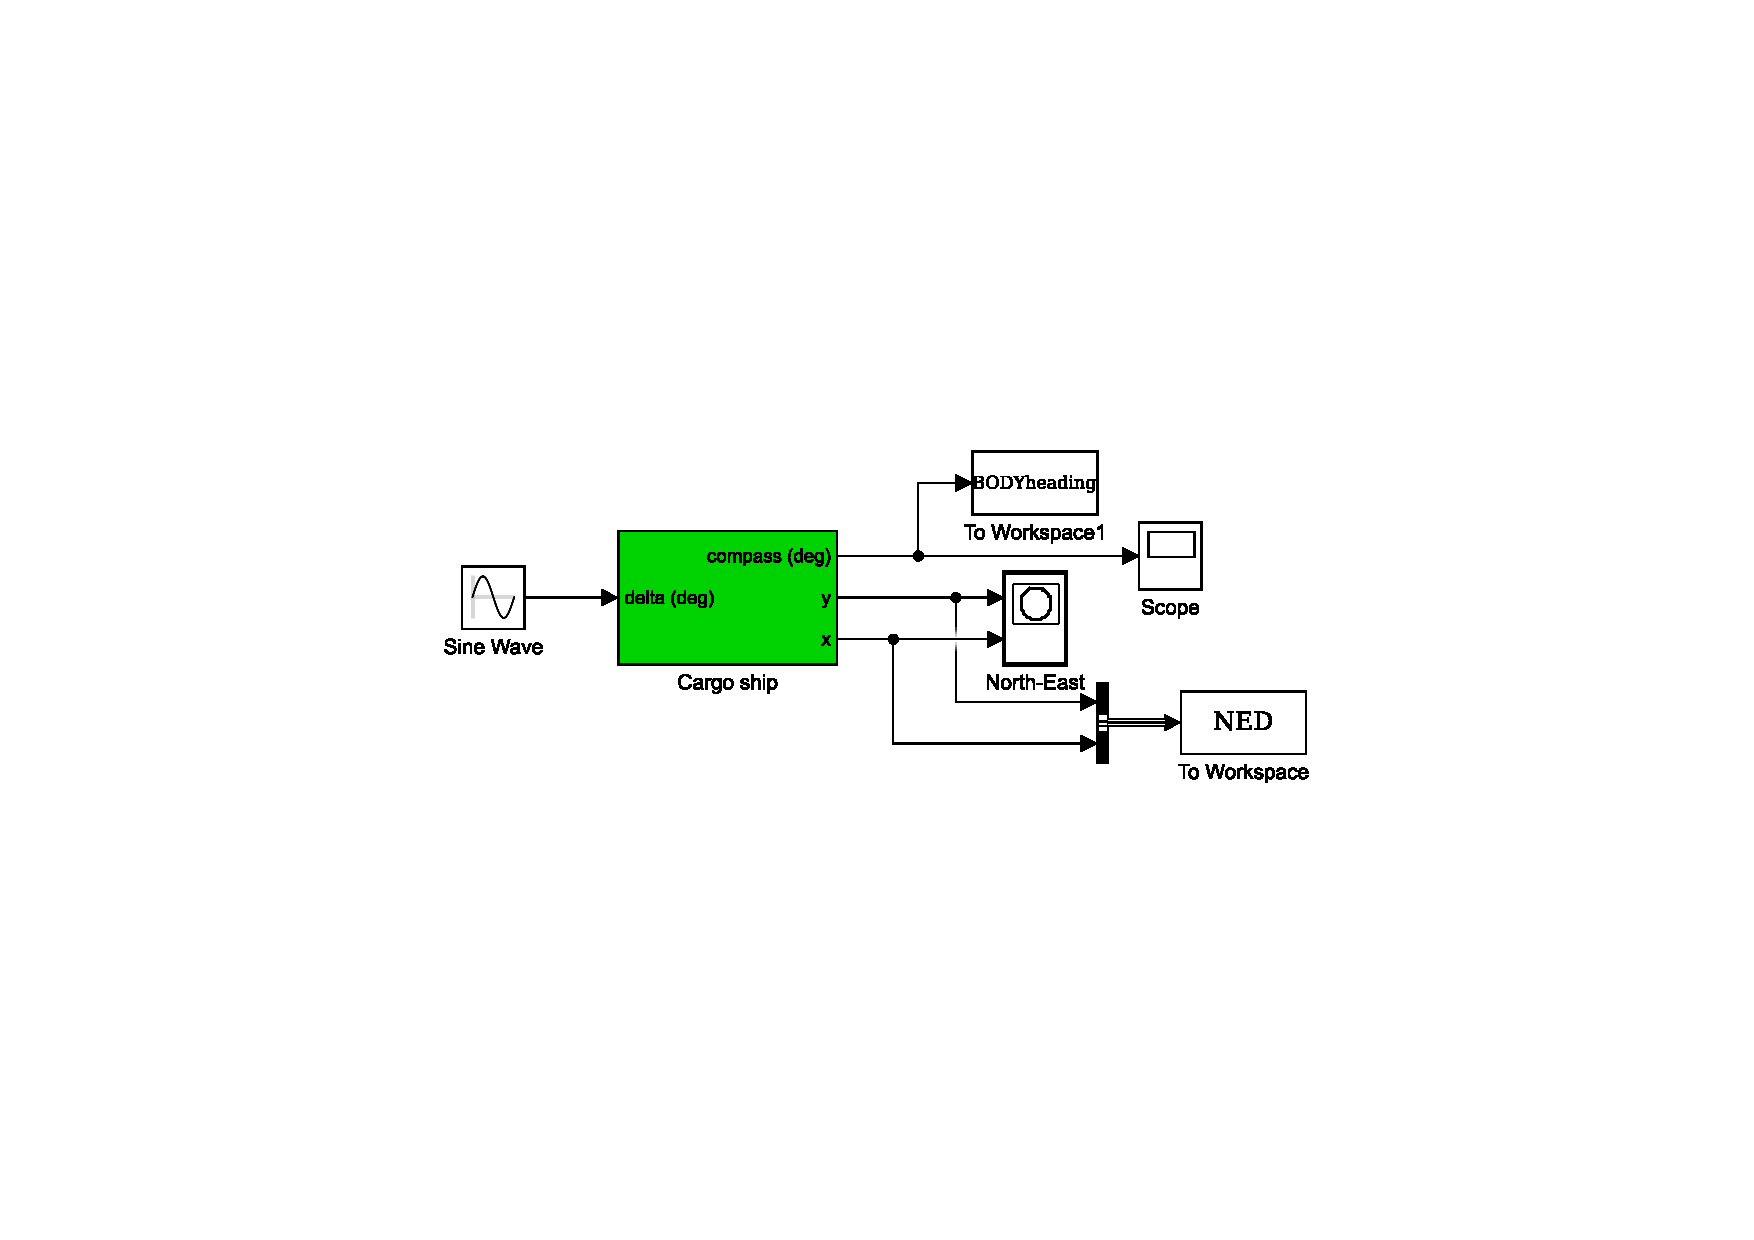
\includegraphics[trim=200 200 200 200, clip, width=\textwidth]{figures/models/p5p1b_c_model.pdf}
	\caption{Handed out cargo-ship system with sine wave input and measurements on output.}
\label{fig:p5p1b_c_model}
\end{figure}

\begin{figure}[!htb]
	\centering
	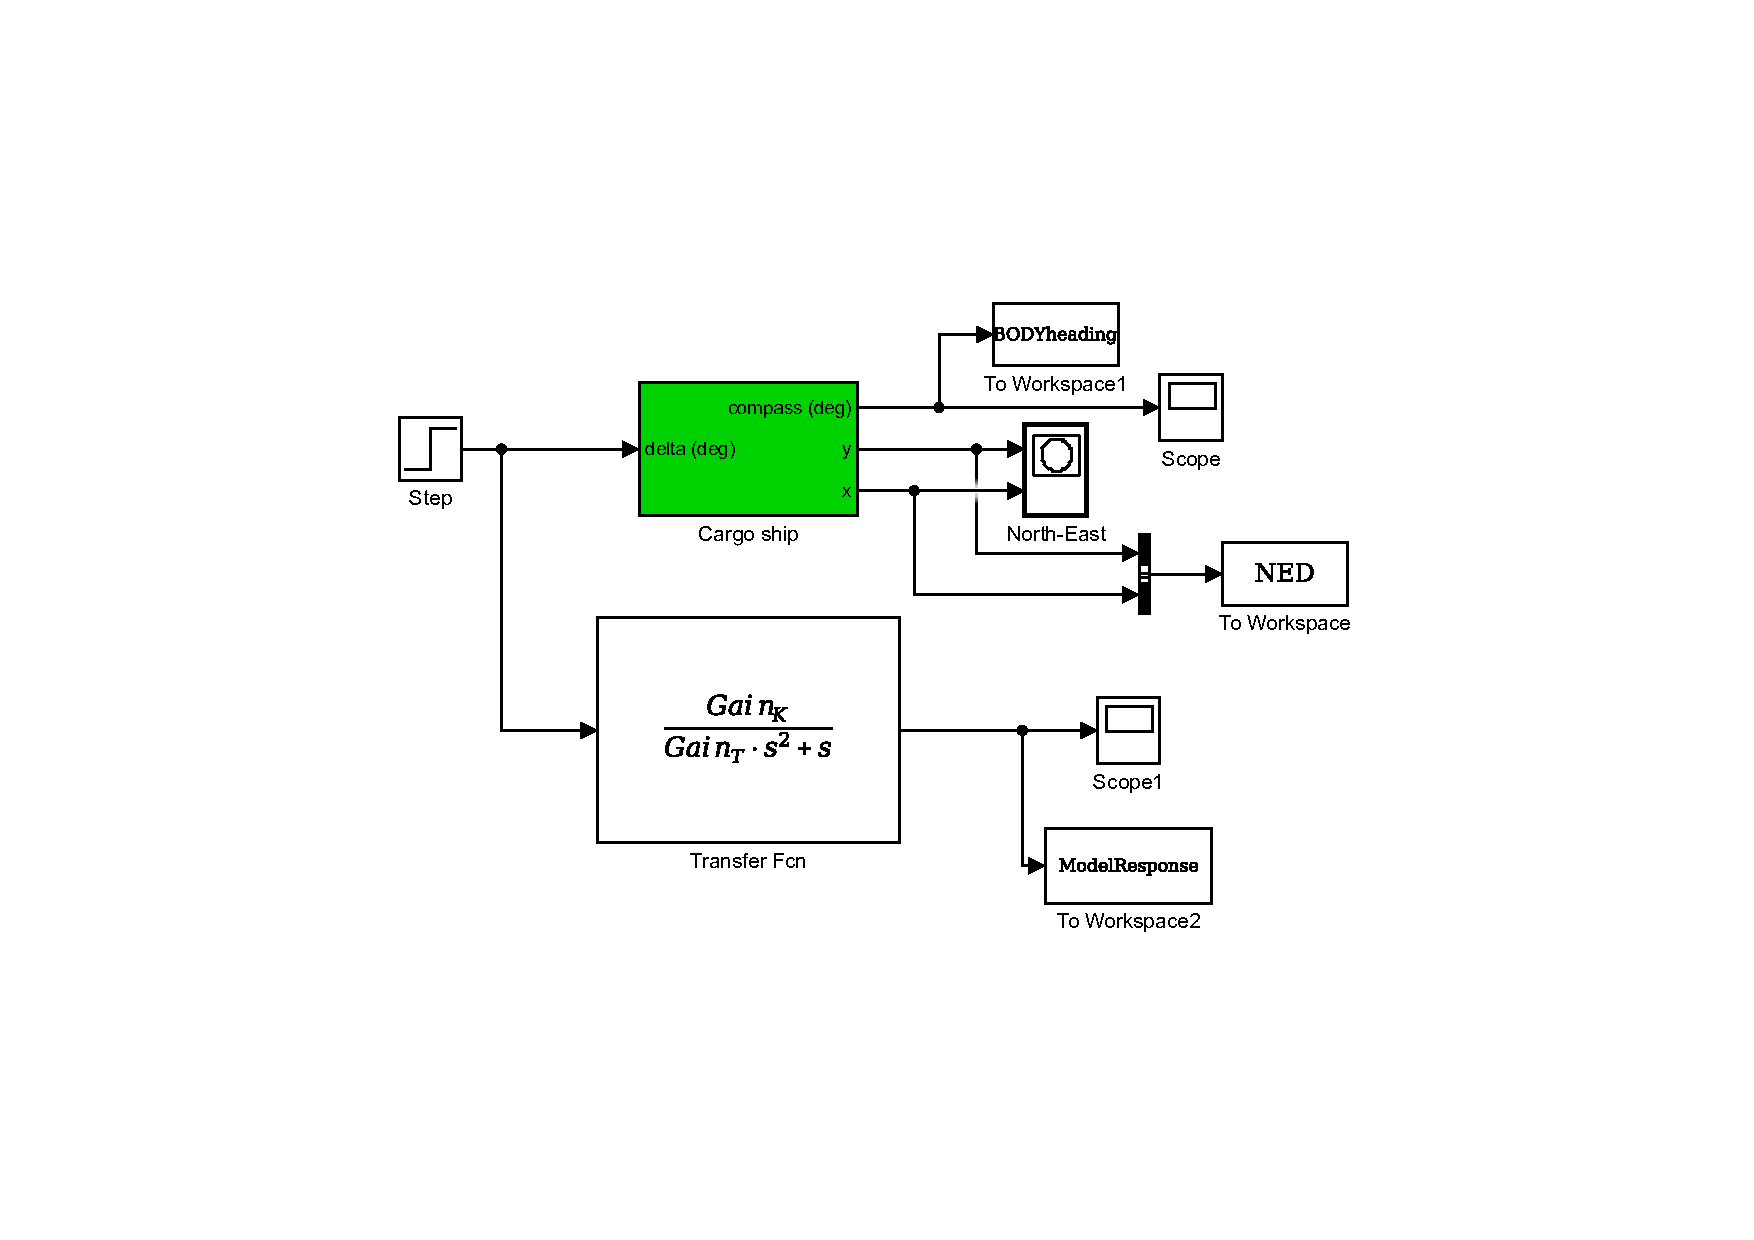
\includegraphics[trim=150 150 150 125, clip, width=\textwidth]{figures/models/p5p1d_model.pdf}
	\caption{Comparison of simulated cargo ship system with theoretical model.}
\label{fig:p5p1d_model}
\end{figure}

\begin{figure}[!htb]
	\centering
	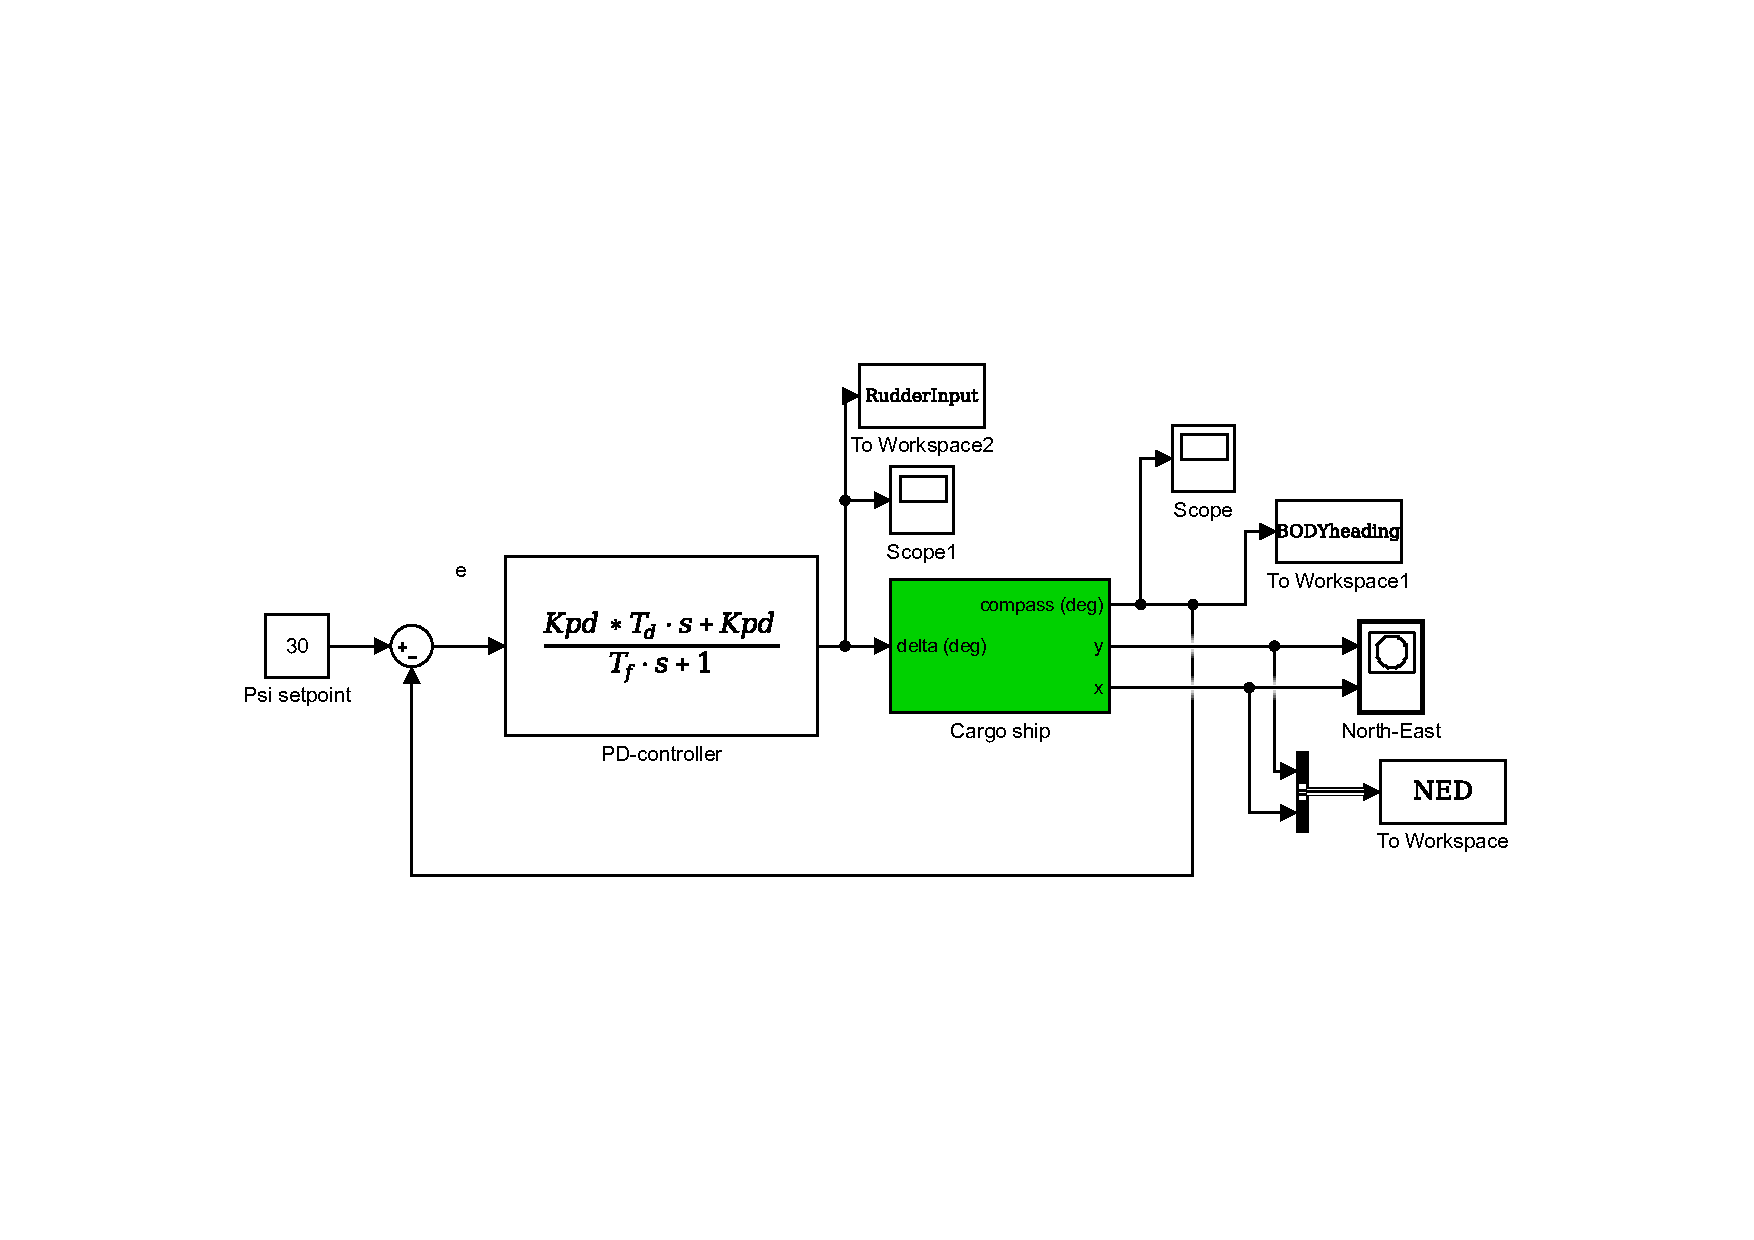
\includegraphics[trim=125 150 100 150, clip, width=\textwidth]{figures/models/p5p3_model.pdf}
	\caption{Cargo-ship system with PD-controller.}
\label{fig:p5p3_model}
\end{figure}

\begin{figure}[!htb]
	\centering
	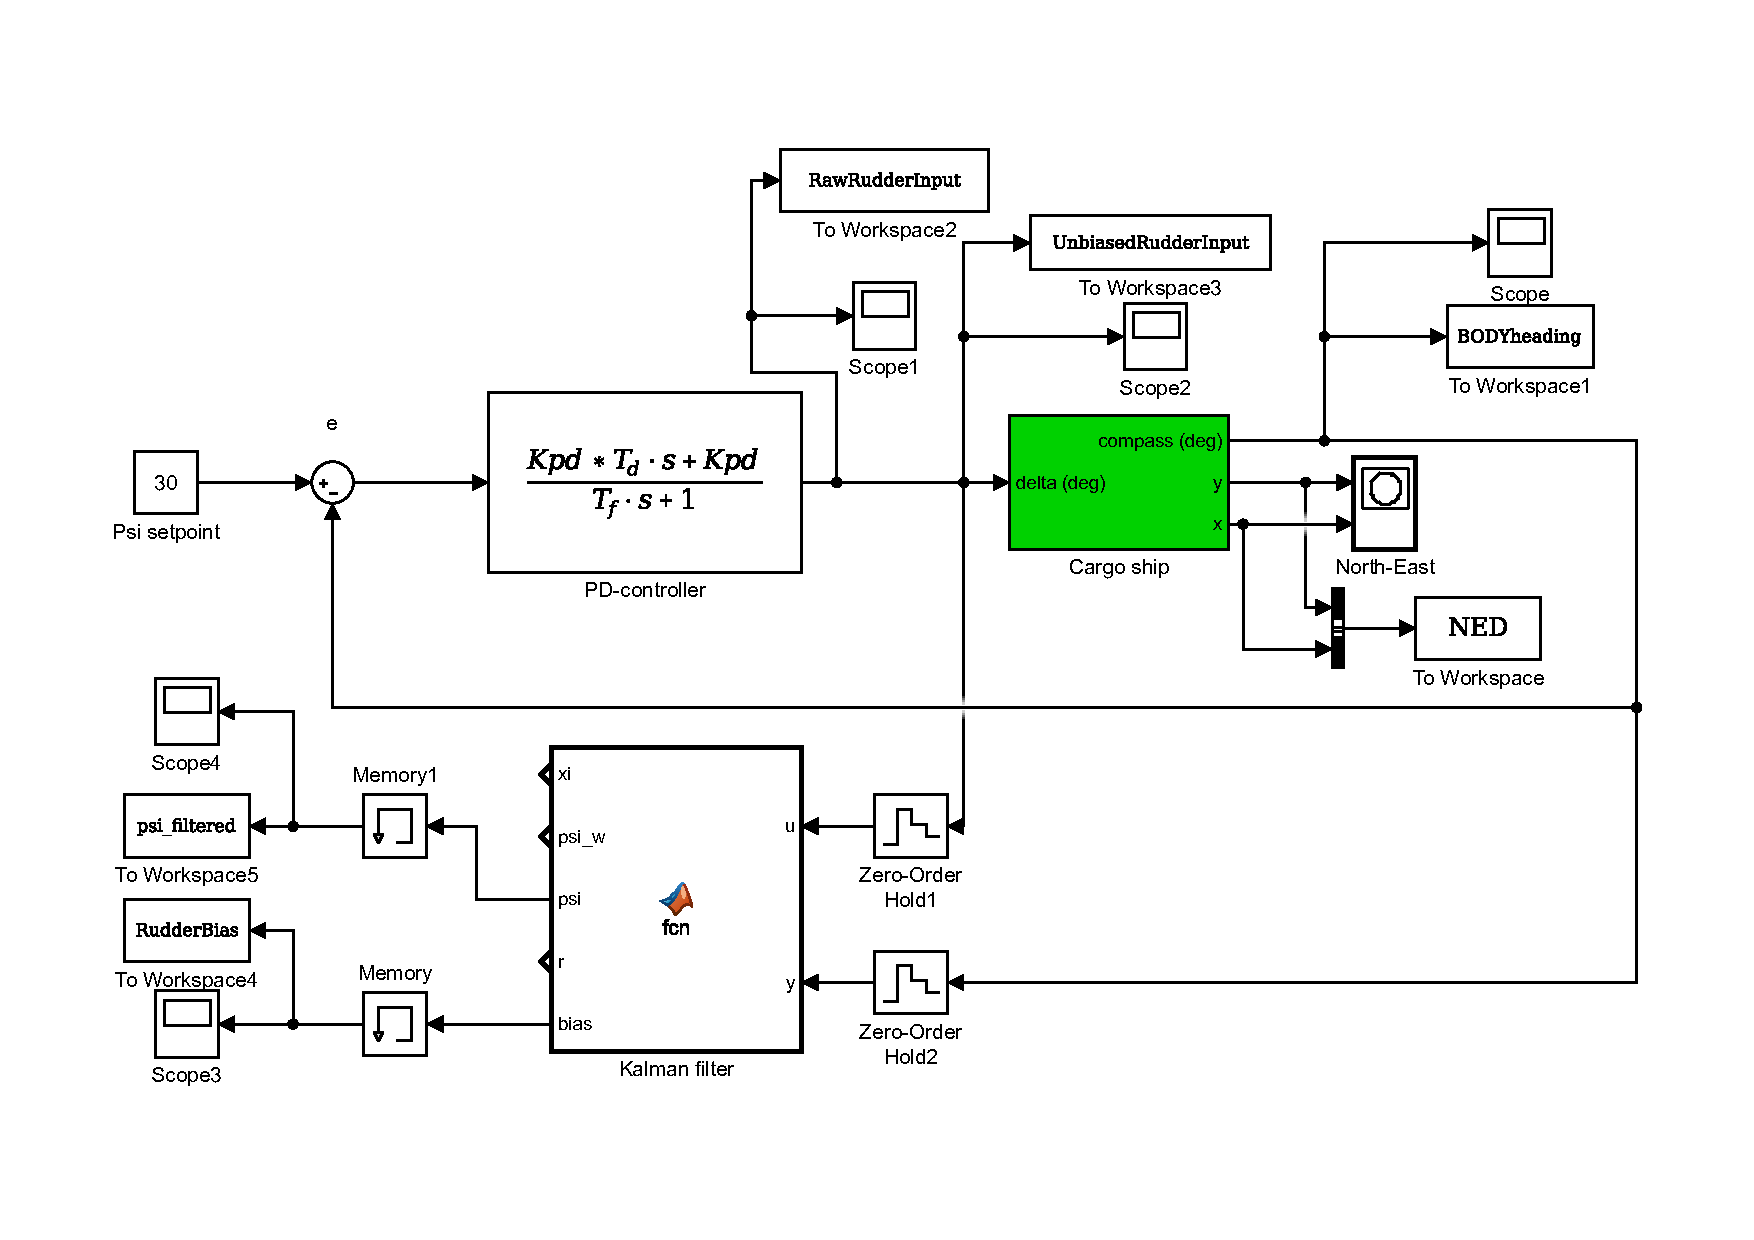
\includegraphics[trim=50 75 25 50, clip, width=\textwidth]{figures/models/p5p5c_model.pdf}
	\caption{Cargo-ship system with PD-controller and Kalman filter.}
\label{fig:p5p5c_model}
\end{figure}

\begin{figure}[!htb]
	\centering
	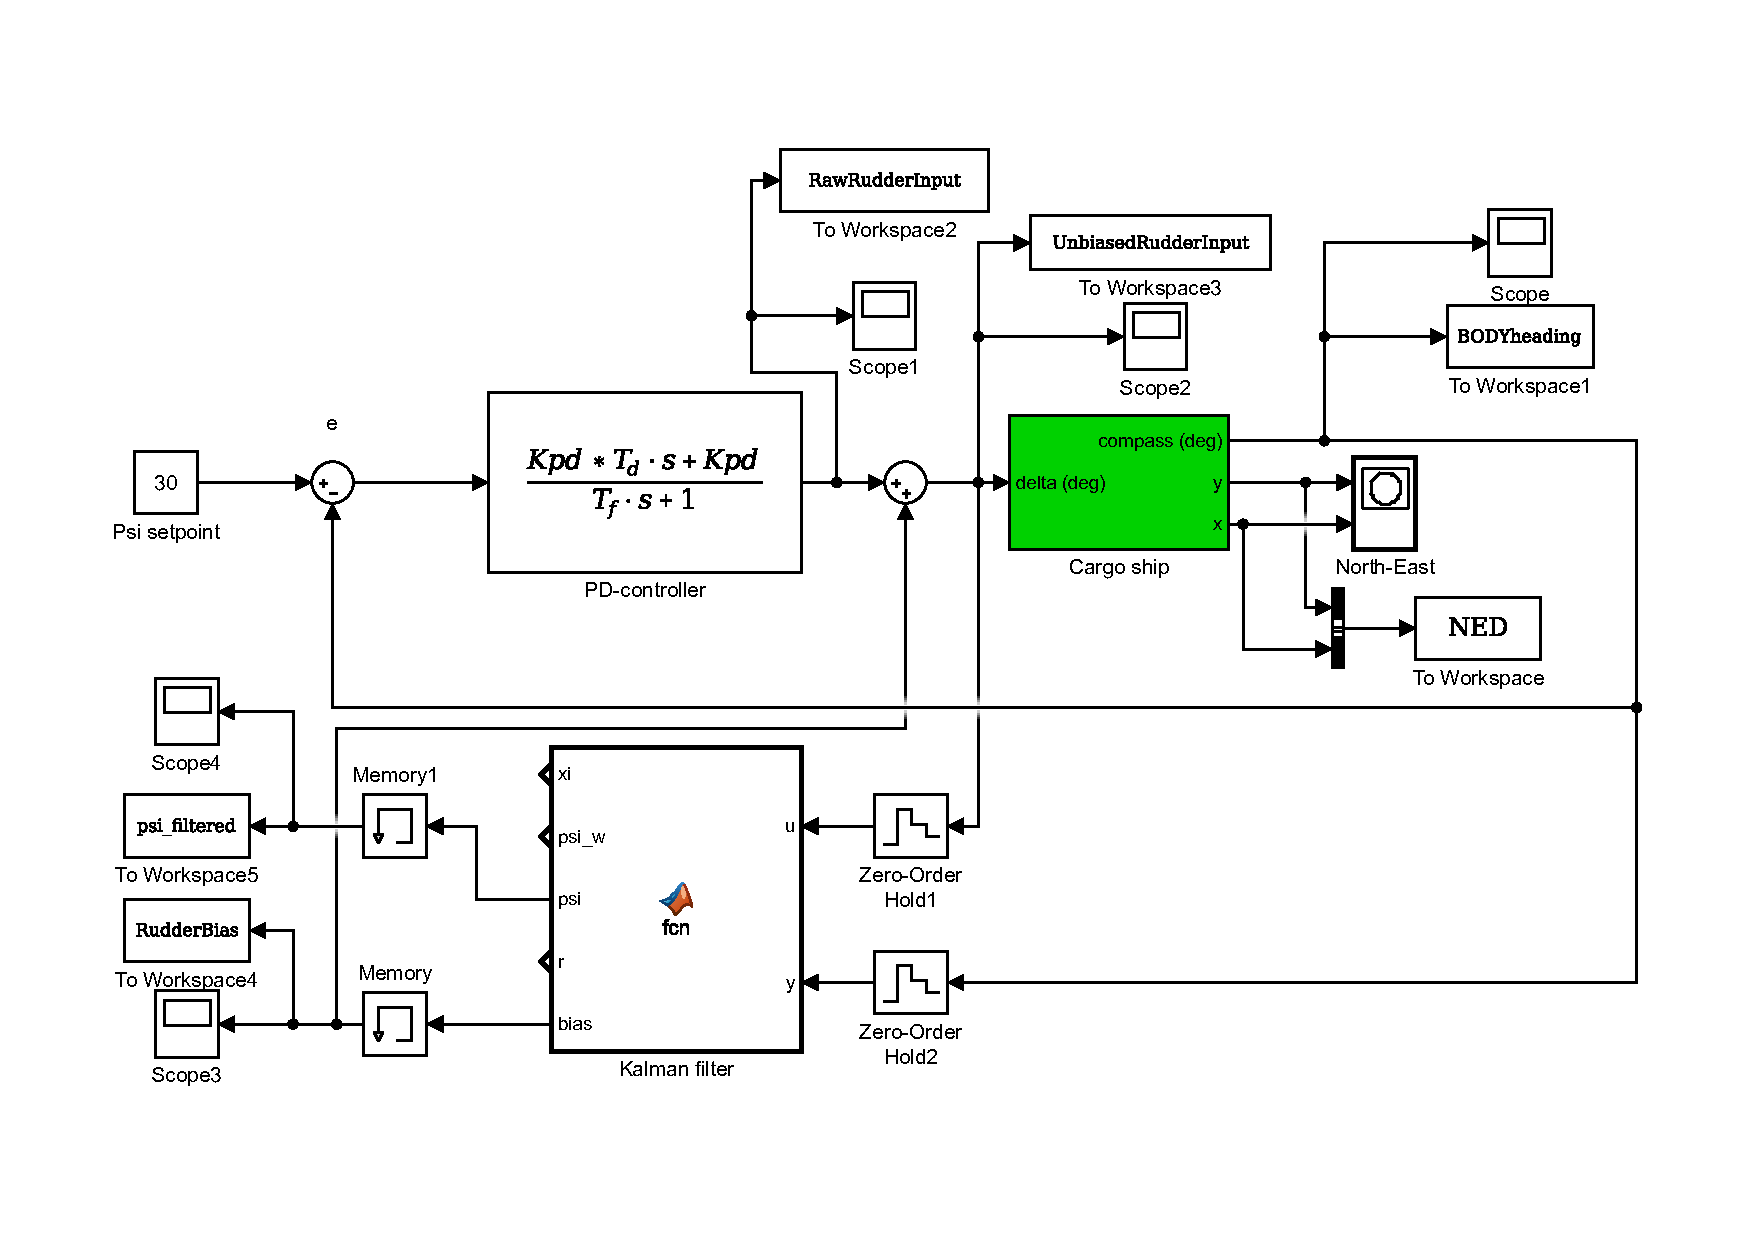
\includegraphics[trim=50 75 25 50, clip, width=\textwidth]{figures/models/p5p5d_model.pdf}
	\caption{Cargo-ship system with PD-controller and Kalman filter and rudder-bias compensation.}
\label{fig:p5p5d_model}
\end{figure}

\begin{figure}[!htb]
	\centering
	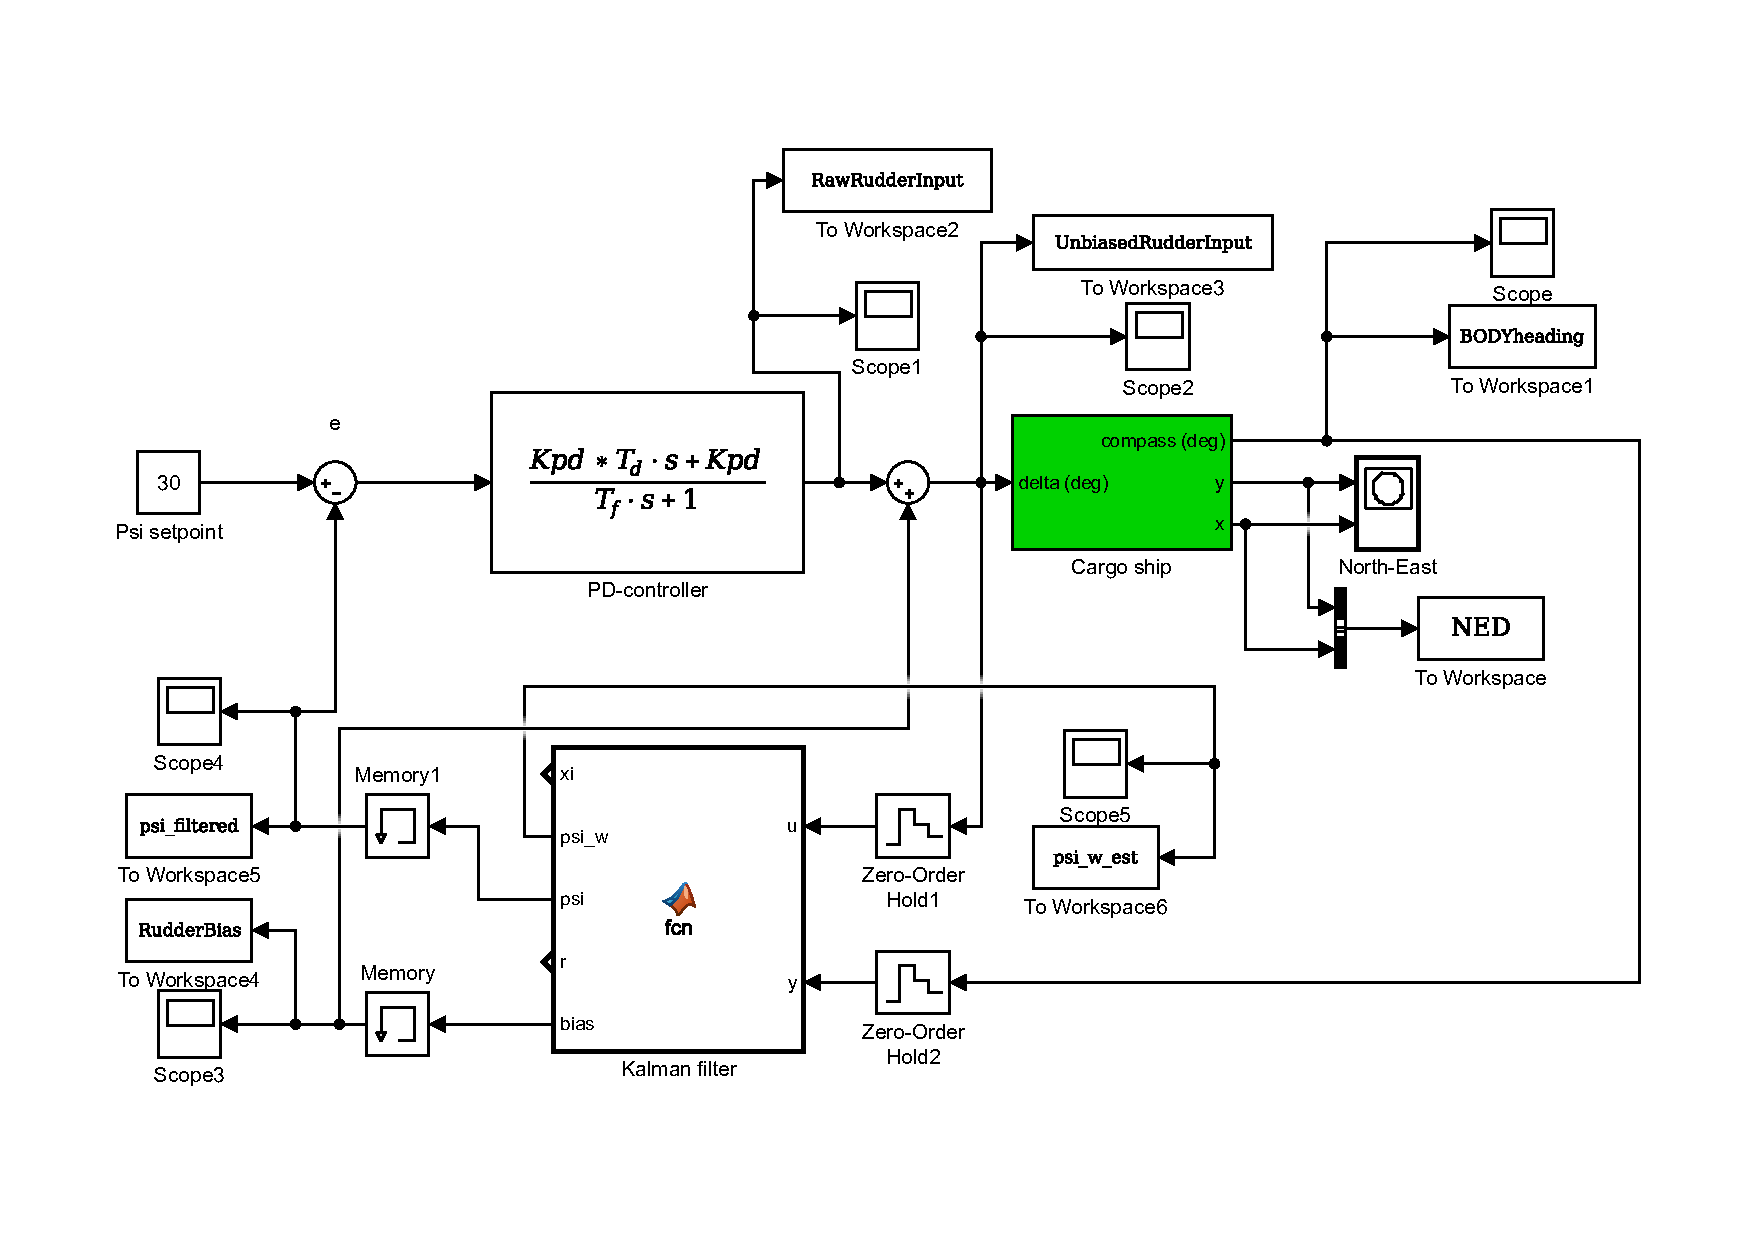
\includegraphics[trim=50 75 25 50, clip, width=\textwidth]{figures/models/p5p5e_model.pdf}
	\caption{Cargo-ship system with PD-controller and Kalman filter, rudder-bias compensation and wave filtering.}
\label{fig:p5p5e_model}
\end{figure}